\documentclass{article}

% if you need to pass options to natbib, use, e.g.:
%     \PassOptionsToPackage{numbers, compress}{natbib}
% before loading neurips_2019

% ready for submission
% \usepackage{neurips_2019}

% to compile a preprint version, e.g., for submission to arXiv, add add the
% [preprint] option:
%     \usepackage[preprint]{neurips_2019}

% to compile a camera-ready version, add the [final] option, e.g.:
     \usepackage[final]{neurips_2019}

% to avoid loading the natbib package, add option nonatbib:
%     \usepackage[nonatbib]{neurips_2019}

\usepackage[utf8]{inputenc} % allow utf-8 input
\usepackage[T1]{fontenc}    % use 8-bit T1 fonts
\usepackage{hyperref}       % hyperlinks
\usepackage{url}            % simple URL typesetting
\usepackage{booktabs}       % professional-quality tables
\usepackage{amsfonts}       % blackboard math symbols
\usepackage{nicefrac}       % compact symbols for 1/2, etc.
\usepackage{microtype}      % microtypography
\usepackage{graphicx}
\usepackage{float}
\usepackage{rotating}

\title{
  Person recognition based on footstep sounds using a deep convolutional neural network\\
  \vskip 0.25in 
  \vskip -\parskip
  Lépéshang alapú személyfelismerés mély konvolúciós neurális hálóval
}
  % The \author macro works with any number of authors. There are two commands
% used to separate the names and addresses of multiple authors: \And and \AND.
%
% Using \And between authors leaves it to LaTeX to determine where to break the
% lines. Using \AND forces a line break at that point. So, if LaTeX puts 3 of 4
% authors names on the first line, and the last on the second line, try using
% \AND instead of \And before the third author name.

\author{%
  Kristóf Rácz \\
  PhD student\\
  Géza Pattantyús-Ábrahám Doctoral School of Mechanical Engineering Sciences\\
  Budapest University of technology and Economics, Faculty of Mechanical Engineering, \\
  Department of Mechatronics, Optics and Engineering Informatics\\
  \texttt{racz.kristof@mogi.bme.hu} \\
}

\begin{document}

\maketitle

\begin{abstract}
  Biometrics are methods to identify persons based on their biological features. From these, gait is one of the best features to use: it can be measured without any extra action from the person, and it is difficult to fake and mask. There have been attempts in the past use a small subset of information available from gait as data for identification: the sound of footsteps. Many methods have been proposed but none of them uses deep learning to solve the problem. Here, a solution is presented for the problem using a deep convolutional neural network (InceptionV3), which achieves a 98\% accuracy in identifying the persons based on their footstep sounds.
\end{abstract}

\renewenvironment{abstract}%
{%
  \vskip 0.075in%
  \centerline%
  {\large\bf Absztrakt}%
  \vspace{0.5ex}%
  \begin{quote}%
}
{
  \par%
  \end{quote}%
  \vskip 1ex%
}

\begin{abstract}
  A biometrika azon módszerek gyűjtőfogalma, amelyek az egyes személyeket biológiai tulajdonságaik alapján igyekszik azonosítani. Ezek közül a tulajdonságok közül a járáskép mondható az egyik legmegbízhatóbb módszernek: az azonosítandó személy külön beavatkozása nélkül mérhető, és e mellett kifejezetten nehéz megváltoztatni vagy imitálni. A múltban már volt példa arra, hogy a járáskép egy kis alhalmazát, a járás hangját alkalmazzák emberek felismerésére. Több módszer is megjelent, azonban ezek közül egyik sem alkalmazta a deep learning technikáját. Jelen dokumentumban a feladat egy mély konvolúciós hálót (InceptionV3) alkalmazó megoldás kerül bemutatásra, mely 98\%-os pontosságot ért el a személyek járáshang alapú azonosításának feladatában.
\end{abstract}

\section{Introduction}
Biometrics can be used to identify people: from our fingerprints and iris to our DNA, numerous biological parameters can be used to identify a person (\textsc{Chinegaram, 2017}). Security systems use this to control who has access to important places or information (e.g. unlocking our phone or pc via a fingerprint sensor), and Surveillance systems have been known to track people by recognizing their face. However, these systems are not infallible: contact lenses for iris scanners, printed silicon fingerprints for fingerprint scanners, masks for face recognition or voice recording for voice detection. However, it's also been shown numerous times, that a person's gait (the way he/she walks) is unique for all individuals. Using gait as
a biometric identifier has some key advantages:

\begin{itemize}
  \item{It can be detected visually (using cameras), or by the vibrations it generates (microphones for the generated sound, or sensors recording mechanical vibrations), without interrupting the activities of the person}
  \item{It is difficult to replicate an other person's patterns}
  \item {It is also difficult to mask one's gait patterns. This could provide more reliable tracking in surveillance systems, as hiding or changing one's face is much easier than hiding one's walking patterns.}
\end{itemize} 

Identifying someone based on the vibrations their steps generate could prove useful in today's world of smart devices. For example a corridor instrumented with vibration sensors could be used to unlock doors for the right person without interrupting their flow at all.

Although the research presented here deals with footstep sound recorded with a microphone, the principles and processes would be easily adaptable to seismic data: the only difference is the media through which the vibrations reach the sensor, and the sensors themselves.

\section{Literature}

A number of studies have explored the topic of identifying people based on footstep sounds. In 1999 \textsc{Tanaka} and \textsc{Inoue} recorded footsteps on a tile floor using a single microphone. They were able to achieve an 83\% recognition rate by extracting the pitch frequency and first peak frequency of footsteps and performing what is essentially K-means clustering. It's not exactly clear as to what this recognition rate is in reference to though, whether it is for recognizing people, or recognizing footwear.

\textsc{Shoji et al.} preformed a similar experiment in 2005, where they used one microphone to record the footsteps of five persons wearing slippers. They used mel-cepstrum analysis to extract a feature vector from the recordings, and applied the k-means method to these. No clear overall accuracy is given for recognizing the persons.

In 2014 \textsc{Geiger et al.} achieved 65.5\% recognition rate on a large database of 305 subjects using hidden markov models. In 2017 \textsc{Guo and Wang} implemented a Bayesian decision classifier for samples in noisy environments, resulting in a more robust classifier than previous works, which is able to achieve over 80\% accuracy in ideal conditions. 

\textsc{Mukhopadhyay et al.} used a different approach on recording in 2018: they used geophones (vibration sensors) to collect footstep data. Using a Gaussian support vector machine, they were able to achieve a 92.29\% accuracy.

Also in 2018, \textsc{Riwurohi et al.} used a multi-microphone setup for data collection, calculated Mel Frequency Cepstrum Coefficients from the recordings, and used a Feed forward neural network with 5 inputs (minimum, maximum, mean, standard deviation and median values of the cepstrum) and 2 hidden layers. They achieved 98.7\% accuracy.

\section{Methods}
\subsection{Data}
\subsubsection{Data collection}
Data was collected in the Motion Laboratory of the Department of Mechatronics, Optic and Engineering Informatics. 

The recordings of footstep sound were collected from 6 individuals, with a total of 32 individual shoe - person combinations (including socks). For each combination a total of 20 takes were recorded (except for one case with only 19 takes). One take consisted of the person walking from the edge of the room towards the microphones in a straight line. The recording was stopped when the person reached the microphones. This took them between 3 and 7 steps.

The recording equipment was lent by the Kármán Studio, including: a dynamic (Shure SM58) and a condenser (AudioTechnica AT2020)
microphone, a small mixer and a usb sound card, as well as the required cables and microphone stands. The signal from the two microphones were recorded simultaneously on the stereo tracks of the recordings (one microphone recorded only to the right, the other only to the left channel). The data was recorded using Audacity\footnote{https://www.audacityteam.org} on a 64 bit Windows 10 machine at a rate of 44.1 kHz, and 32 bit resolution. The recording setup can be seen on \textit{figure \ref{fig:rec_setup}}. A sample of the equipment and environment noise was also recorded by recording a few seconds in 'silence'.

\begin{figure}[ht]
  \centering
  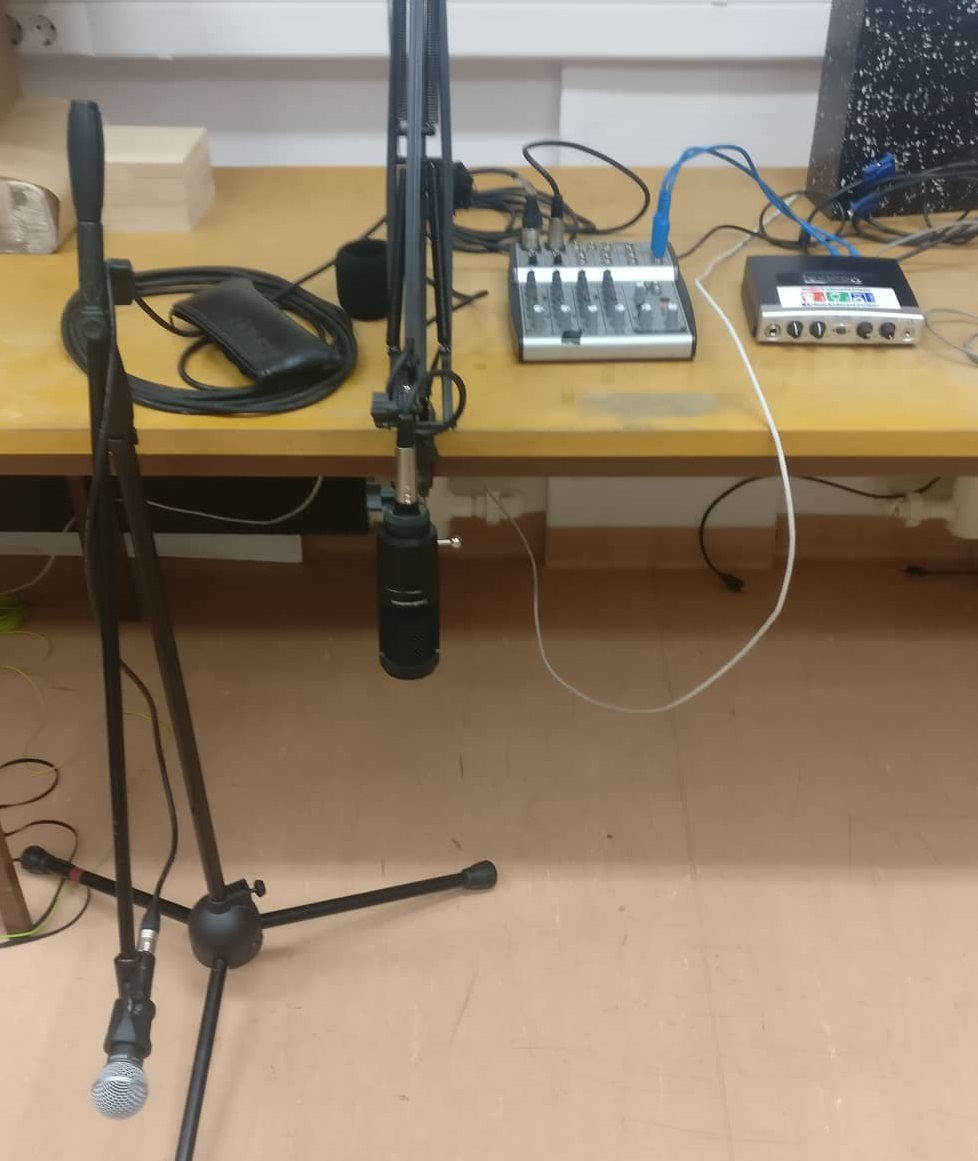
\includegraphics[width=0.6\textwidth]{img/recording_setup}
  \caption{Audio recording setup with two microphones, a mixer and an USB sound card}
  \label{fig:rec_setup}
\end{figure}

\subsubsection{Data preprocessing}
Each take was exported to an individual \verb+*.wav+ file with the naming scheme \verb+ID_shoeType_Take#.wav+. A python scrip was used to process these files into mel spectrograms. Only the recordings of the AudiTechnica microphone was used. The script performed the following steps to process the audio files (all Butterworth filters were second order):

\begin{enumerate}
  \item load the recording of environment and equipment noise data
  \item separate the mono track of the noise profile of the AudioTechnica microphone from the recording
  \item filter the noise profile with a Butterworth highpass filter ($f_{cutoff} = 1 kHz$) filter
  \item iterate through the recordings in the input directory:
  \begin{enumerate}
    \item load the next recording and separate the mono channel of the AudioTechnica microphone
    \item apply a noise reduction based on the noise profile
    \item apply a Butterworth highpass filter ($f_{cutoff} = 100 Hz$) filter
    \item apply a Butterworth notch filter ($f_{cutoff} = 45 Hz$, $width = 2 Hz$) filter
    \item calculate the mel spectrogram using the \verb+librosa+ package
    \item plot the spectrogram using \verb+matplotlib+
    \item save the spectrogram to a file in the appropriate train/validate/test folder based on the take number of the original file (takes 1-16 go to train, 17-18 to validate and 19-20 to test data)
  \end{enumerate}
\end{enumerate}

An example of the output can be seen in \textit{figure \ref{fig:mel_spect}}.

\begin{figure}[ht]
  \centering
  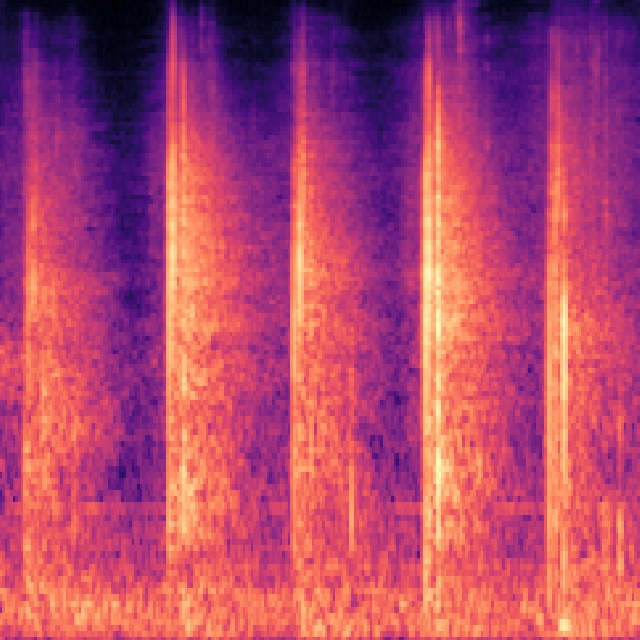
\includegraphics[width=0.4\textwidth]{img/hiveMind_slippers_12}
  \caption{Example mel spectrogram output of data preprocessing}
  \label{fig:mel_spect}
\end{figure}

\subsection{Model}
I choose the \verb+InceptionV3+ (\textsc{Szegedy et al. 2015}) convolutional neural network as the basis for my model. The top part of the model is replaced with a dense feed forward network to classify the data into 6 classes (as per the 6 persons whose footsteps were recorded). The structure of this part is determined based on hyperparameter optimization, with the following general structure:

\begin{enumerate}
  \item input layer from InceptionV3, with a shape of (6, 6, 2048)
  \item a pooling layer
  \begin{itemize}
    \item \verb+GlobalMaxPooling()+
    \item \verb+GlobalAveragePooling()+
    \item \verb+None+
  \end{itemize}
  \item a flatten layer
  \item 1 to 3 hidden dense layers, with each having
  \begin{itemize}
    \item 8, 16, 32, 64, 128, 256 or 512 neurons (independent of the other dense layers)
    \item an activation function: \verb+ReLU+, \verb+LeakyReLU+ or \verb+Swish+ (\textsc{Ramachandran et al. 2017})
    \item a normalization layer: either \verb+BatchNormalization+ before activation, or \verb+Dropout+ after activation
  \end{itemize}
  \item an output dense layer with 6 neurons and \verb+Softmax+ activation
\end{enumerate}

In addition, the following parameters related to training the model:
\begin{itemize}
  \item an optimizer
  \begin{itemize}
    \item \verb+Adam+ or \verb+SGD+
    \item A learning rate of $0.01$, $0.001$ or $0.0001$
  \end{itemize}
  \item a \verb+batch_size+ of 4, 8, 16, 32, 64, 128 or 256
\end{itemize}

\subsection{Training}
I tried to follow the general steps of transfer learning on a CNN, but training the classification model on the bottleneck features of InceptionV3 with the ImageNet wights proved to be of little use: it was clear that the feature extraction needed for the spectrograms is different than what is used for normal photographs. Based on this, my strategy for training the model was the following:

\begin{enumerate}
  \item pretrain \verb+InceptionV3+ for feature extraction on spectrograms:
  \begin{enumerate} 
    \item put an arbitrary classifier on top (\verb+Flatten, Dense(126, activation='relu'),+ \verb+Dense(32, activation='relu'), Dense(6, activation='softmax')+)
    \item Train the model on the train dataset, validate with validation dataset
    \item Save trained weights of \verb+InceptionV3+
  \end{enumerate}
  \item generate bottleNeck features from the data with the pretrained \verb+InceptionV3+
  \item perform hyperparameter optimization with \verb+keras-tuner+ on the dense classification network using the generated bottleneck features
  \item train the selected classification architecture on the bottleneck features
  \item join \verb+InceptionV3+ with the pretrained wights to the trained classification network
  \item train the complete model on the data to fine-tune everything
\end{enumerate}

\section{Results}
\subsection{Hyperparameter optimization}

The newly released \verb+keras-tuner+ framework was used to perfrom a hyperparameter otimization using the HyperBand algorithm (\textsc{Li and Jamieson, 2018}). The hyperparameters of the first 20 best performing models can be seen in \textit{table \ref{tab:hyperopt}}. I did not find an easy way to also get the metrics related to the performance metrics of the models, such as their validation accuracy and loss, the time it took to complete one epoch of training, and the total number of epoch before stopping.

Based on the first 20 models, the parameters that really matter are the:
\begin{itemize}
  \item  pooling, from which no pooling layer is the best
  \item  the regularization layer, where Dropout is a clear winner over using BatchNorm
  \item  the optimizer, from which SGD with a learning rate of 0.0010 is the most common
\end{itemize}
For the rest of the hyperparameters the following values were selected  with the goal of minimizing the number of parameters to train:
\begin{itemize}
  \item  Swish activation function
  \item  1 hidden layer with 64 neurons
  \item  A batch\_size of 16
\end{itemize}

Due to an error in defining the model which resulted in only having 0.1 tested as the dropout rate, I've run an additional round of hyperparameter optimization, this time with hyperparameters selected above, and a dropout rate between 0.1 and 0.5, with 0.005 steps. There was no really significant difference, but the results showed that 0.2 is the best value for this parameter.

The complete model has total of 26\,521\,830 parameters, of which 21\,802\,784 belong to InceptionV3, and 4\,719\,046 belong to the selected fully connected classifier.

\begin{sidewaystable}
  \caption{Hyperparameters of the first 20 models}
  \label{tab:hyperopt}
  \centering
  \begin{tabular}{lllllllllll}
    \toprule
    Place   & Pooling    & Activation     & Regularization & learning\_rate & Optimizer  & batch\_size & nLayers & nNeurons\_0 & nNeurons\_1 & nNeurons\_2 \\
    \midrule
    0       & None       & Swish          & Dropout        & 0.0100         & SGD        & 16          & 2       & 128         & 16          & 16.0   \\
    1       & None       & LeakyReLU      & Dropout        & 0.0010         & SGD        & 8           & 2       & 256         & 64          & 128.0  \\
    2       & None       & ReLU           & Dropout        & 0.0010         & SGD        & 64          & 2       & 64          & 64          & 256.0  \\
    3       & None       & LeakyReLU      & Dropout        & 0.0010         & SGD        & 8           & 2       & 256         & 64          & 128.0  \\
    4       & None       & LeakyReLU      & Dropout        & 0.0010         & Adam       & 128         & 2       & 256         & 16          & 128.0  \\
    5       & None       & LeakyReLU      & Dropout        & 0.0010         & SGD        & 32          & 3       & 64          & 256         & 128.0  \\
    6       & None       & ReLU           & Dropout        & 0.0010         & SGD        & 64          & 2       & 64          & 64          & 256.0  \\
    7       & None       & LeakyReLU      & Dropout        & 0.0010         & SGD        & 128         & 2       & 128         & 8           & 64.0   \\
    8       & None       & ReLU           & Dropout        & 0.0010         & SGD        & 256         & 3       & 256         & 512         & 128.0  \\
    9       & None       & LeakyReLU      & Dropout        & 0.0010         & SGD        & 32          & 3       & 64          & 256         & 128.0  \\
    10      & None       & Swish          & Dropout        & 0.0001         & SGD        & 16          & 2       & 256         & 16          & 64.0   \\
    11      & None       & Swish          & Dropout        & 0.0010         & Adam       & 16          & 1       & 64          & 16          & 32.0   \\
    12      & None       & LeakyReLU      & Dropout        & 0.0010         & SGD        & 8           & 2       & 256         & 64          & 128.0  \\
    13      & None       & Swish          & Dropout        & 0.0010         & Adam       & 32          & 1       & 256         & 8           & 128.0  \\
    14      & None       & Swish          & Dropout        & 0.0001         & SGD        & 16          & 2       & 256         & 16          & 64.0   \\
    15      & None       & Swish          & Dropout        & 0.0010         & Adam       & 16          & 1       & 64          & 16          & 32.0   \\
    16      & None       & Swish          & Dropout        & 0.0001         & SGD        & 32          & 2       & 512         & 16          & 64.0   \\
    17      & None       & Swish          & Dropout        & 0.0100         & SGD        & 16          & 2       & 128         & 16          & 16.0   \\
    18      & None       & ReLU           & Dropout        & 0.0010         & SGD        & 256         & 3       & 256         & 512         & 128.0  \\
    19      & None       & Swish          & Dropout        & 0.0001         & Adam       & 64          & 1       & 32          & 128         & 256.0  \\
    \bottomrule
  \end{tabular}
\end{sidewaystable}

\subsection{Training}

As described earlier, the classification model was trained on the bottleneck features first, and then the whole model was trained on the original data. The evaluation of the final model resulted on the metrics reported in \textit{table \ref{tab:eval_results}}. The confusion-matrix fo the predictions can be seen on \textit{figure \ref{fig:conf_matrix}}. In summary, the network only misclassified a single sample from the test dataset, which can be considered very good. With these results it is among, if not the best performing solution for identifying people based on their footstep sounds compared with the literature.

\section{Conclusion}

The trained model performed the task excellently, maybe even too well. It could be an indication that it's much more complex than it needs to be, or the data is too homogeneous. I am planning on collecting more data from new persons, and seeing how many classes can the model handle.

\begin{table}[!h]
  \caption{Evaluation metrics of the model}
  \label{tab:eval_results}
  \centering
  \begin{tabular}{lc}
    \toprule
    Metric & Value \\
    \midrule
    Test accuracy:  & 0.98 \\
    Test loss:      & 0.0462 \\
    Test precision: & 0.976 \\
    Test recall:    & 0.983 \\
    Test f1\_score:  & 0.978 \\
    Number of misclassified samples: & 1 \\
    \bottomrule
  \end{tabular}
\end{table}

\begin{figure}[!h]
  \centering
  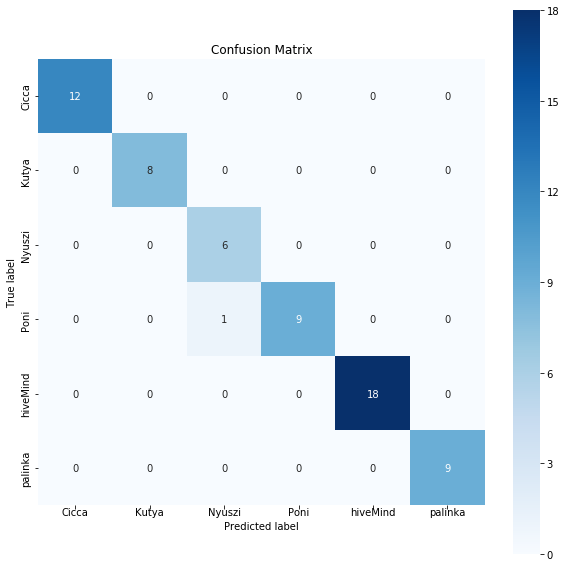
\includegraphics[width=0.7\textwidth]{img/conf_matrix}
  \caption{Confusion matrix for the test samples}
  \label{fig:conf_matrix}
\end{figure}

Another option is to streamline the architecture os InceptionV3. The input originally consist of colored images, spectrograms however, by nature, can be represented as grayscale images. The first layers of the network could be modified accordingly. It'd also be interesting to explore if the depth of the convolutional model can be reduced without loosing performance.

Another interesting challenge would be to split the data in a different manner, based on shoe types. Assign one shoe type as validation, an other shoe type as test (preferably the socks option, as intuitively that is the hardest type to predict, as the amount of information is minimal, the footsteps are very quiet). Unfortunately, as some persons only recorded with three shoes, this would make the data even more sparse than it already is.

\section*{References}

\small

Chinegaram, K.\ (2017) Various Biometric Authentication Techniques: A Review. {\it Journal of Biometrics \& Biostatistics} {\bf 8} (5):371.

Geiger, J. T.\ \& Kneißl, M.\ \& Schuller, B.\ \& Rigoll, G. (2014) Acoustic gait-based person identification using hidden markov models. {\it MAPTRAITS 2014 - Proceedings of the 1st ACM Audio/Video Mapping Personality Traits Challenge and Workshop, Co-located with ICMI 2014} pp. 25-30

Guo, F.\ \& Wang, X.\ (2017) Robust footstep identification system based on acoustic local features. {\it IET Biometrics} {\bf 6} (6):387-392

Li, L.\ \&, Jamieson, K.\ (2018) Hyperband: A Novel Bandit-Based Approach to Hyperparameter Optimization.  {\it Journal of Machine Learning Research} {\bf 18} (185):1-52.

Mukhopadhyay, B.\ \& Anchal, S.\ \& Kar, S.\ (2018) Person Identification using Seismic Signals generated from Footfalls. {\it arXiv:1809.08783}

Ramachandran, P.\ \& Zoph, B.\ \& Le, Q.\ (2017) Swish: a Self-Gated Activation Function. {\it arXiv:1710.05941.}

Riwurohi, J. E.\ \& Istiyanto, J. E.\ \& Mustofa, K.\ \& Putra, A. E.\ (2018) People Recognition through Footstep Sound Using MFCC Extraction Method of Artificial Neural Network Back Propagation. {\it International Journal of Computer Science and Network Security} {\bf 18} (4):28-35

Shoji, Y.\ \& Itai, A.\ \& Yasukawa, H.\ (2005) Personal identification using footstep detection in in-door environment. {\it IEICE Transactions on Fundamentals of Electronics, Communications and Computer Sciences} {\bf E88-A} (8):2072-2076

Szegedy, C.\ \& Vanhoucke, V.\ \$ Ioffe, S.\ \& Shlens, J.\ \& Wojna, Z.\ (2015) Rethinking the Inception Architecture for Computer Vision {\it arXiv:1512.00567.}

Tanaka, M.\ \& Inoue, H.\ (1999) A Study on walk-recognitions by frequency analysis of footsteps. {\it EEJ Transactions on Electronics, Information and Systems} {\bf 119} (6):762-763

\end{document}
